\documentclass[11pt]{article}
\usepackage{lmodern,setspace,amsmath,amssymb,amsfonts,amsthm,graphicx,multicol,grffile,float}
\usepackage{mathtools}
\usepackage{authblk,url,csvsimple,cuted,dblfloatfix,parskip}
\usepackage[a4paper, top=0.9in, bottom=1.05in, left=1.01in, right=1.01in]{geometry}
\usepackage[polish]{babel}
\usepackage[utf8]{inputenc}
\usepackage[unicode]{hyperref}
\usepackage{listings}
\usepackage{booktabs}

\usepackage[linesnumbered,ruled,vlined]{algorithm2e}
\DontPrintSemicolon
\SetKw{Break}{break}
\SetKw{Continue}{continue}
\DeclareMathOperator*{\argmax}{arg\!max}
\DeclareMathOperator*{\argmin}{arg\!min}

\title{PTSZ - Zadanie 1 - Problem $Q5 | r_j | F$}
\author{Dariusz Max Adamski 136674 (grupa I9, godzina 8:15)}
\affil{dariusz.adamski@student.put.poznan.pl}
\date{Data oddania: \today}

\def\code#1{\texttt{#1}}

\begin{document}

\maketitle

\section*{Wstęp}

W tym sprawozdaniu opisane jest podejście rozwiązujące problem szeregowania zadań na pięciu równoległych maszynach o różnych prędkościach, z czasami startowymi i minimalizacją średniego czasu przepływu.

\section{Generator instancji}

\begin{algorithm}
\caption{Algorytm generatora instancji dla problemu}
$t \coloneqq 0$ \;
\For{i \in 1 \dots n}{
    \If{i = 0 \lor \text{Bernoulli}(0.05)}{
        $\mu_p \coloneqq  \text{Uniform}(10, 100)$ \;
        $\sigma_p \coloneqq \text{Uniform}(5, 20)$ \;
        $\mu_s \coloneqq \text{Uniform}(1, 4)$ \;
    }
    $t \coloneqq t + \lfloor \text{Normal}(\mu_s, 0.5\mu_s) \rfloor$ \;
    $r_i \coloneqq \max \{ 0, \lfloor  \text{Normal}(t, 0.5*\mu_p) \rfloor \}$ \;
    $p_i \coloneqq \text{clip}(\lfloor \text{Normal}(\mu_p, \sigma_p) \rfloor, 1, 200)$ \;
}
Potasuj losowo zadania
\end{algorithm}

\begin{figure}[h]
\caption{Wizualizacje wygenerowanych instancji o wielkości 100, 200 i 400}
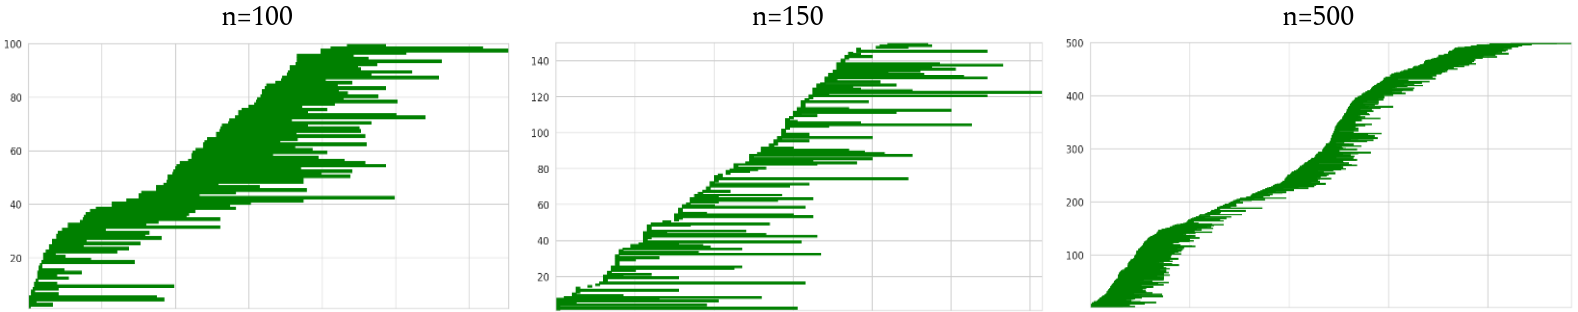
\includegraphics[width=\textwidth]{inst.png}
\centering
\end{figure}

\subsection{Opis algorytmu}

Funkcja generująca instancje działa na zasadzie symulacji śledzącej aktualny czas $t$. Generowane jest $n$ zadań z czasem rozpoczęcia $r_i$ i czasem przetwarzania $p_i$. Przed wygenerowaniem każdego zadania, czas symulacji jest zwiększany o krok losowany z rozkładu normalnego wyśrodkowanego na parametrze $\mu_s$ z odchyleniem standardowym $0.5\sigma_s$.
Czas przetwarzania jest losowany z rozkładu normalnego o średniej wartości $\mu_p$ i odchyleniu standardowym $\sigma_p$, przy czym minimalną wartością jest 1 a maksymalną 200.
Następnie generowany jest czas rozpczęcia $r_j$, który jest losowany z rozkładu normalnego wyśrodkowanego na aktualnym czasie symulacji $t$, z odchyleniem standardowym równym połowie aktualnego średniego czasu przetwarzania $0.5\mu_p$, przy czym minimalną wartością $r_j$ jest 0.
Po wygenerowaniu wszystkich zadań, zadania są tasowane.
Szybkości maszyn $b_m$ są ustawione na 1, 0.25, 0.4, 0.65 i 0.8.

Najciekawszą według mnie częścią algorytmu jest to, że ani krok symulacji, ani parametry zadań nie są losowane ze stałych rozkładów prawdopodobieństwa, ale z rozkładów których parametry losowo zmieniają się z prawdopodobieństwem 5\%. Średni czas przetwarzania zadania $\mu_p$ jest na przykład losowany z rozkładu jednostajnego ciągłego z minimalną wartością 10 a maksymalną 100. Podobnie odchylenie standardowe czasu przetwarzania $\sigma_p$ i średni krok czasowy $\mu_s$ są losowane z rozkładów jednostajnych. Takie podejście sprawia, że dane instancji są wielomodowe, co widać po okresowych zmianach właściwości zadań. Na rysunku 1. zamieściłem wizualizacje kilku wygenerowanych instancji, które pokazują tą charakterystykę.

\section{Algorytm szeregowania}

\begin{algorithm}
\caption{Algorytm dla problemu szeregowania}
$h(j, m) = \alpha_1(r_j - t_m) + \alpha_2\frac{p_j}{b_j}$ \;
$\forall_{m \in M}  t_m \coloneqq 0$ \;
$t \coloneqq 0$ \;
\While{T \neq \varnothing}{
$T_{\text{valid}} \coloneqq \{\langle j, m \rangle \in T \times M \mid t_m \leq t \land r_j \leq t \}$ \;
    \If{T_{\text{valid}} = \varnothing}{
        \uIf {$\forall_j t < r_j$}{
            $t \coloneqq \min_j r_j$ \;
        }
        \Else {
            $t \coloneqq \min_m t_m$ \;
        }
        \Continue \;
    }
$\langle j, m \rangle \coloneqq T_{\text{valid}}[ \argmin_i h(T_{\text{valid},i}) ]$ \;


$t_m \coloneqq \max\{ r_j, t_m \} + \frac{p_j}{b_m}$ \;
Zaplanuj zadanie $j$ na maszynie $m$ \;
$T \coloneqq T \setminus \{ T_j \}$ \;
}
\end{algorithm}

\subsection{Oznaczenia}

Zbiór $T$ początkowo zawiera wszystkie zadania $T_1 \dots T_n$. Gdy zadanie jest dodane do uszeregowania, usuwane jest z tego zbioru.
Zbiór $M$ zawiera numery maszyn od 1 do 5.
Zmienna $t$ oznacza aktualny czas symulacji, a zmienne $t_i$ oznacza aktualny czas symulacji na i-tej maszynie.

\subsection{Opis algorytmu}

Algorytm szeregowania działa w następujący sposób. Dla danego punktu w czasie symulacji $t$ wybierana jest najlepsza według heurystyki para zadania i maszyny. Rozpatrywane są tylko maszyny, których czas jest mniejszy lub równy aktualnemu czasowi $t_m \leq t$ (do tej maszyny w tym momencie nic nie możemy przypisać), oraz zadania, których czas rozpoczęcia jest mniejszy lub równy aktualnemu czasowi $r_j \leq t$ (nie chcemy, żeby maszyna skoczyła do czasu $r_j$ w przyszłości, bo zostawiłaby dziurę w uszeregowaniu, którą byśmy musieli później zapełnić).

Po wybraniu zadania $j$ i maszyny $m$ obliczany jest nowy czas maszyny $t_m$, z uwzględnieniem jej szybkości $b_m$, zadanie jest dodane do uszeregowania na tej maszynie, a następnie jest usuwane ze zbioru $T$.

Wybrana heurystyka priorytetyzuje najmniejszy czas wykonania zadania, w zależności od maszyny $p_j/b_m$ i najbardziej spóźnione/najwcześniej dostępne zadania $r_j - t_m$. Heurystyka jest sparametryzowana wartościami $\alpha$, które są losowane z zakresu (0, 1). Najlepsze parametry ustalane są przez uruchomienie algorytmu 20 razy. Tylko najlepszy wynik szeregowania jest zapisywany.

\subsection{Analiza złożoności}

Złożoność algorytmu to $O(n^2)$, gdzie $n$ to wielkość instacji - liczba zadań. Złożoność wynika z tego, że zachłannie planujemy $n$ zadań, a przy planowaniu każdego zadania rozważamy maksymalnie $5n$ zadań kandydatów, aby skonstruować zbiór $T$, Jeśli zbiór kandydatów jest pusty, to ustawiamy aktualny czas na najmniejszy czas maszyny $t_m$, dzięki czemu złożoność algorytmu nie zależy od czasów $p_i, r_i$. Na złożoność nie wpływa fakt, że stałą liczbę razy uruchamiam algorytm, żeby dostosować parametry heurystyki. 

\end{document}
